\documentclass[a4paper, twoside, 10pt]{report}

%% Language and font encodings
\usepackage[english]{babel}
\usepackage[utf8]{inputenc}
\usepackage[T1]{fontenc}

%% Sets page size and margins
\usepackage[a4paper,top=3cm,bottom=2cm,left=3cm,right=3cm,marginparwidth=1.75cm]{geometry}

%% Useful packages
\usepackage[backend=biber,style=imperialharvard]{biblatex}
\usepackage{afterpage}
\usepackage{amsmath}
\usepackage{amsthm}
\usepackage{csquotes}
\usepackage{enumitem}
\usepackage{graphicx}
\usepackage{lipsum}
\usepackage{booktabs}

\usepackage{titlesec}

% Listings (for displaying code):
\usepackage{listings}
\lstset{
    frame = single, 
    framexleftmargin=15pt
}

% Center figure captions:
\usepackage[labelfont=bf,justification=centering]{caption}

% ----------- Algorithm2e setup
\usepackage[ruled,vlined]{algorithm2e}
\makeatletter
\renewcommand{\SetKwInOut}[2]{%
  \sbox\algocf@inoutbox{\KwSty{#2}\algocf@typo:}%
  \expandafter\ifx\csname InOutSizeDefined\endcsname\relax% if first time used
    \newcommand\InOutSizeDefined{}\setlength{\inoutsize}{\wd\algocf@inoutbox}%
    \sbox\algocf@inoutbox{\parbox[t]{\inoutsize}{\KwSty{#2}\algocf@typo:\hfill}~}\setlength{\inoutindent}{\wd\algocf@inoutbox}%
  \else% else keep the larger dimension
    \ifdim\wd\algocf@inoutbox>\inoutsize%
    \setlength{\inoutsize}{\wd\algocf@inoutbox}%
    \sbox\algocf@inoutbox{\parbox[t]{\inoutsize}{\KwSty{#2}\algocf@typo:\hfill}~}\setlength{\inoutindent}{\wd\algocf@inoutbox}%
    \fi%
  \fi% the dimension of the box is now defined.
  \algocf@newcommand{#1}[1]{%
    \ifthenelse{\boolean{algocf@inoutnumbered}}{\relax}{\everypar={\relax}}%
%     {\let\\\algocf@newinout\hangindent=\wd\algocf@inoutbox\hangafter=1\parbox[t]{\inoutsize}{\KwSty{#2}\algocf@typo\hfill:}~##1\par}%
    {\let\\\algocf@newinout\hangindent=\inoutindent\hangafter=1\parbox[t]{\inoutsize}{\KwSty{#2}\algocf@typo:\hfill}~##1\par}%
    \algocf@linesnumbered% reset the numbering of the lines
  }}%
\makeatother
% --------- end algorithm2e setup

% \bm allows typing bold math:
\usepackage{bm}

% -------- Fancy page headers:
\usepackage{fancyhdr}
\pagestyle{fancy}
\fancyhf{}
\rhead{\slshape\nouppercase\leftmark}
\lhead{\slshape\nouppercase{\rightmark}}
\renewcommand{\headrulewidth}{1pt}
\renewcommand{\footrulewidth}{1pt}

\lfoot{\thepage}
\rfoot{\thepage}
% -------- Finish setting up fancy page headers


% ---------- Setup for definitions:
\usepackage{tipa}
\usepackage{tcolorbox}
\definecolor{mdgrey}{rgb}{0.8, 0.8, 0.8}
\usepackage[framemethod=tikz]{mdframed}
\usepackage{lipsum}
\newtheoremstyle{defi}
  {\topsep}%
  {\topsep}%
  {\normalfont}%
  {}%
  {\bfseries}% 
  {:}%
  {.5em}%
  {\thmname{#1}\thmnote{~(#3)}}%
\theoremstyle{defi}
\newmdtheoremenv{definitioni}{Definition}
\newmdtheoremenv[
hidealllines=true,
leftline=true,
innertopmargin=0pt,
innerbottommargin=0pt,
linewidth=4pt,
linecolor=gray!40,
innerrightmargin=0pt,
]{definitionii}{Definition}
\newmdtheoremenv[
roundcorner=5pt,
innertopmargin=0pt,
innerbottommargin=5pt,
linewidth=4pt,
linecolor=gray!40,
]{definitioniii}{Definition}
% ---------- End setup for definitions

\usepackage[colorinlistoftodos]{todonotes}

\usepackage{xcolor}
\definecolor{sussexgreen}{HTML}{003b4a}

\usepackage[colorlinks=true, allcolors=sussexgreen]{hyperref}

\renewcommand*{\rmdefault}{bch}
\renewcommand*{\ttdefault}{lmtt}
\newcommand{\citationneeded}{\textcolor{red}{[citation-needed]}}

\DeclareMathOperator*{\argmin}{\arg\!\min}
\DeclareMathOperator*{\argmax}{\arg\!\max}

\title{Compression of Natural Language}

% Uncomment if you want a subtitle:
% \vspace{1em}\large Interim Report}

\author{Guy Aziz\\267649}
% Update supervisor and other title stuff in title/title.tex

% Add bigger skip between paragraphs, makes reading easier:
\setlength{\parskip}{0.5em}

\bibliography{bibs/bibliography.bib}

\begin{document}
\begin{titlepage}

\newcommand{\HRule}{\rule{\linewidth}{0.5mm}} % Defines a new command for the horizontal lines, change thickness here

%----------------------------------------------------------------------------------------
%	LOGO SECTION
%----------------------------------------------------------------------------------------


\includegraphics[width=8cm]{title/logo.eps}\\[1cm] % Include a department/university logo - this will require the graphicx package
 
%----------------------------------------------------------------------------------------

\center % Center everything on the page

%----------------------------------------------------------------------------------------
%	HEADING SECTIONS
%----------------------------------------------------------------------------------------

\textsc{\LARGE Individual Project}\\[1.5cm] % Name of your university/college
\textsc{\Large University of Sussex}\\[0.5cm] % Major heading such as course name
\textsc{\large School of Engineering and Informatics}\\[0.5cm] % Minor heading such as course title

%----------------------------------------------------------------------------------------
%	TITLE SECTION
%----------------------------------------------------------------------------------------
\makeatletter
\HRule \\[0.6cm]
{ \huge \bfseries \@title}\\[0.6cm] % Title of your document
\HRule \\[1.5cm]
 
%----------------------------------------------------------------------------------------
%	AUTHOR SECTION
%----------------------------------------------------------------------------------------

\begin{minipage}{0.4\textwidth}
\begin{flushleft} \large
\emph{Author:}\\
\@author % Your name
\end{flushleft}
\end{minipage}
~
\begin{minipage}{0.4\textwidth}
\begin{flushright} \large
\emph{Supervisor:} \\
Prof. Ian Mackie \\[1.2em] % Supervisor's Name
%\emph{Second Marker:} \\
%Mr. Edward Hyde % second marker's name
\end{flushright}
\end{minipage}\\[2cm]
\makeatother

% If you don't want a supervisor, uncomment the two lines below and remove the section above
% \Large\@author\\[3cm] % Your name

%----------------------------------------------------------------------------------------
%	DATE SECTION
%----------------------------------------------------------------------------------------

{\large \today}\\[2cm] % Date, change the \today to a set date if you want to be precise

\vfill % Fill the rest of the page with whitespace

\end{titlepage}

% \begin{abstract}
% Your abstract goes here
% \end{abstract}
% 
% \renewcommand{\abstractname}{Acknowledgements}
% \begin{abstract}
% Thanks mum!
% \end{abstract}

\tableofcontents


% Redefine the chapter title format
\titleformat{\chapter}[block]
  {\normalfont\huge\bfseries} % format
  {\thechapter.} % label (chapter number)
  {1em} % separation between label and title
  {} % before-code


% Inputs:
% Uncomment or add folders to add your own chapters and input files.

\chapter{Introduction}

Human language contains many redundancies and regularities. It is possible, for example, for a person to infer from an incomplete sentence a missing letter or word, or to spot an error through an inconsistency between text and context.

This is done, first, through the abstraction of an underlying, concise representation of the text, and then through a re-generation of the elaborated text from the conceptual understanding. In humans, one's ability to induce a general pattern and deduce its application to a specific case in this way is often an indication of their comprehension of a text, and of having a grasp of the underlying meaning.

Because of this, it is believed by some researchers (most notably Marcus Hutter) that the ideal lossless compression of a text would require comprehension, and that the first is therefore an AI-complete problem.

This project aims to explore the relationship between compression and comprehension.

To view the code used in this project, visit \url{https://github.com/Guy29/FYP}.

\section{Motivation}
\label{sec:motivation}

Occam’s razor is a general principle in science and rationality commonly attributed to William of Ockham (1290-1349) which states “entities should not be multiplied beyond necessity”, usually interpreted to mean “the simplest theory is usually the correct one.”

It is easy to take this principle for granted, as it seems to work in both science and in our daily experience. But why this should be the case, i.e. why we live in a regular enough world that simpler models of it tend to be more correct than more complex ones, is not obvious, and it has been historically pointed out by many philosophers (most famously David Hume) that knowledge gained in this way stands on shaky foundations. \autocite{Henderson2018}

Solomonff’s theory of inductive inference provides a formalism for Occam’s razor. It posits an agent making observations in a world that operates by an unknown algorithm, and based on that premise shows that the agent would do well to assume that the length of the algorithm by which its world runs in effect follows a probability distribution that assigns shorter (and therefore simpler) algorithms more probability. This probability distribution is known as the universal prior.

The argument Solomonoff uses can be understood as follows: if the agent considers all algorithms of the same complexity as equally likely, then the algorithms can be divided into subsets where each subset is functionally equivalent. Because there are more ways to implement simpler algorithms than more complex ones, they accrue more probability mass. For example, a crime investigator who knows that Alice likes apple pie and Bob doesn’t may consider the following hypotheses (of equal complexity) for the disappearance of an apple pie:

\begin{enumerate}
    \item Alice stole it, wearing a red shirt.
    \item Alice stole it, wearing a blue shirt.
    \item Bob stole it, after having a change of taste.
\end{enumerate}

If each of these hypotheses is given the same probability initially, based on being of equal complexity, then a grouping of the first two as functionally equivalent (the colour of the shirt being irrelevant) makes it twice as likely that Alice is the culprit.

Solomonoff’s theory of inductive inference uses the concept of Kolomogorov complexity, which refers to the length of the shortest program that would produce a specific output. For example, the Kolomogorov complexity of the string “1111 … 11111” is lower than that of “wp9j8 … fd27c”, as the first is more regular. The actual design of compression algorithms can be thought of as a way of empirically determining the Kolomogrov complexity of data by finding an algorithm that produces it which is shorter than the data itself.

In the same way that Occam’s razor lacked formalism and proof until Solomonoff, the concept of intelligence similarly lacks formalism in modern computer science, and psychologist R. J. Sternberg remarks “there seem to be almost as many definitions of intelligence as there were experts asked to define it.” \autocite{Legg2007}

\textcite{Hutter2000} proposes a formalism of an intelligent agent which he terms AIXI that combines the above ideas as well as ideas from reinforcement learning. AIXI is a theoretical agent which, in each time step,

\begin{enumerate}
    \item Makes an action $a_i$.
    \item Receives an observation $o_i$ and a reward (positive or negative) $r_i$.
    \item Generates all possible algorithms by which its world can run which would have predicted all of its observations and rewards so far, and weighs the probabilities of those algorithms inversely to their length (i.e. it applies the universal prior).
    \item Uses the most likely algorithms (or models of its world) to simulate the world, predict potential observations and rewards for potential future actions, and thereby decide on its following actions to maximize its reward.
\end{enumerate}

It can be seen that the above description of AIXI requires an agent that can effectively create a concise, compressed world-model that generates the observations it has made of its world so far (i.e. arriving at the simplest explanation for the underlying mechanisms of the world it inhabits, where simplicity indicates low Kolmogorov complexity), and that having such a model is most predictive of its success. It is for this reason that Hutter believes that intelligence can be defined in terms of data compression.

Based on this hypothesis, \textcite{Hutter2006} created the Hutter Prize, intended to “encourage development of intelligent compressors/programs as a path to AGI”. The prize rewards improvements in data compression on a specific 1 GB text file, titled \texttt{enwik9}, which is extracted from the English Wikipedia, chosen on the reasoning that “Wikipedia is an extensive snapshot of human knowledge. If you can compress the first 1GB of Wikipedia better than your predecessors, your (de)compressor likely has to be smart(er) [...] while intelligence is a slippery concept, file sizes are hard numbers.”

This project examines some of the intuitions that relate compression and comprehension of natural language, and provides an overview of some of the existing theory and of its practical applications.

\section{Professional and Ethical Considerations}
\label{subsec:bcs}
To the best of my knowledge, there are no professional or ethical considerations, as given by the BCS code of conduct (\url{https://www.bcs.org/membership/become-a-member/bcs-code-of-conduct/}) that would constrain any part of this project. The core of the project is a review and discussion of existing techniques, and practical applications will likely be limited to improvements on compression algorithms. All data used in this project is in the public domain.

\section{Structure of this report}
This report approaches compression of natural language from a few different angles. These approaches share some essential concepts, but each also requires its own bit of background. For readability, I've opted to structure the report in a similar way, giving a high-level overview of essential abstract concepts in the \hyperref[chap:overview]{Overview} chapter but also beginning each section of the \hyperref[chap:investigation]{Investigation} chapter with its own specialized background.
\chapter{Introduction}

\begin{definitionii}
\textbf{\emph{dissertation}}
\textipa{[dis@\super rteiS\super @n]}
% dɪsəʳteɪʃən

\noindent   
A dissertation is a long formal piece of writing on a particular subject, especially for a university degree.

\noindent \emph{He is currently writing a dissertation on the Somali civil war.}

\hfill -- Collins English Dictionary \autocite{Smith1998}
\end{definitionii}

Above you will find a nicely typeset definition.
\lipsum[1-4]
\lipsum[1-4]

\begin{figure}
    \centering
    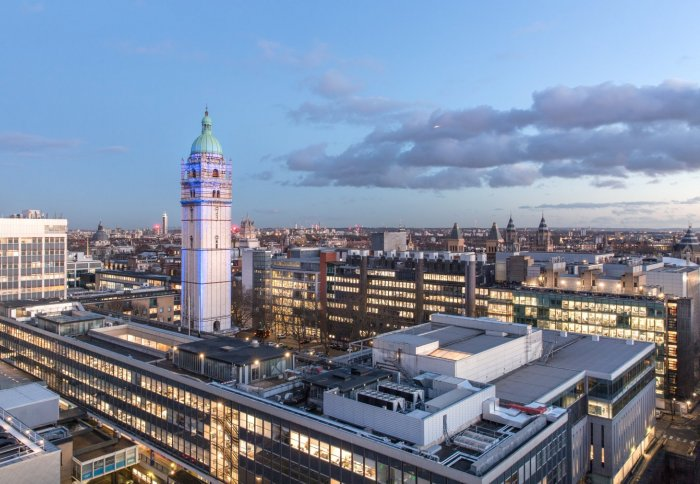
\includegraphics[width=0.8\textwidth]{img/imperial.jpg}
    \caption{Example of including an image}
    \label{fig:imperial-picture}
\end{figure}

\lipsum[2-4] See Figure \ref{fig:imperial-picture}.

\begin{table}[]
    \centering
    \begin{tabular}{llr}  
        \toprule
        \multicolumn{2}{c}{Item} \\
        \cmidrule(r){1-2}
        Animal    & Description & Price (\$) \\
        \midrule
        Gnat      & per gram    & 13.65      \\
                  &    each     & 0.01       \\
        Gnu       & stuffed     & 92.50      \\
        Emu       & stuffed     & 33.33      \\
        Armadillo & frozen      & 8.99       \\
        \bottomrule
    \end{tabular}
    \caption{Example booktabs table. Booktabs tables are nicer than regular ones, in my opinion. This site has a nice GUI for making LaTeX tables, and has a Booktabs option: https://www.tablesgenerator.com/}
    \label{tab:my_label}
\end{table}

\lipsum[1-4] Table \ref{tab:my_label}

\section{Section Example}
\lipsum[1]
\subsection{Subsection Example}
\label{subsection:example}
\lipsum[1]
\subsubsection{Subsubsection Example}

Note that you can reference chapters, sections, subsections and subsubsections. For example: Subsection \ref{subsection:example}

\section{Math Example}

\[
\textrm{score}(x) = \left(\lambda_m\sum_{i=0}^{|\mathbf{m}|} \log \hat{p}_m(d(x, \mathbf{m}_i) \mid l_i)\right) + \left(\lambda_l\sum_{i=0}^{|\mathbf{l}|} \log\hat{p}_l(d(x, \mathbf{l}_i) \mid \mathbf{v}_i)\right) + \lambda_p \hat{p}_p(x)
\]

\section{Algorithm Example}

See Algorithm \ref{algorithm:posit}

\begin{algorithm}[]
\SetAlgoLined
\SetKwInOut{KwInput}{Input}
\SetKwInOut{KwOutput}{Output}
\SetKwInOut{KwPre}{Pre}
\SetKw{Return}{return}
\SetKwProg{Fn}{Function}{}{end}
\LinesNumbered
\KwInput{$\textbf{m}$, such that $\mathbf{m}_i$ is the position of the $i$'th monitor\newline
$\textbf{l}$, such that $\mathbf{l}_i$ is the position of the $i$'th landmark\newline
$\mathbf{p}^m$, such that $\mathbf{p}^m_i$ is the ping latency from monitor $i$ to the target\newline
$\mathbf{p}^l$, such that $\mathbf{p}^l_i$ is the set of ping latencies to landmark $i$}

\BlankLine
\KwPre{Compute $\hat{p}_m(d \mid l)$, an estimator giving the likelihood of the target being distance $d$ away from the monitor, given that the monitor records a latency of $l$ to that target. Implemented by training a KDE using $\mathbf{p}^l$.\newline
Compute $\hat{p}_l(d \mid v)$, an estimator giving the likelihood of the target being distance $d$ away from the landmark, given a Canberra distance of $v$ between the target and the landmark, using training targets.
}
\BlankLine
\KwOutput{Most likely location of the target}
\BlankLine

\Fn{Likelihood($x$, $\mathbf{v}$)} {
MonitorScore $\gets \sum_{i=0}^{|\mathbf{m}|} \log{\hat{p}_m(d(x, \mathbf{m}_i) \mid l_i)}$\;
LandmarkScore $\gets \sum_{i=0}^{|\mathbf{l}|} \log{\hat{p}_l(d(x, \mathbf{l}_i) \mid \mathbf{v}_i)}$\;
\Return MonitorScore + LandmarkScore
}

\BlankLine
$\mathbf{v} \gets $\{$\mathrm{canberra\_distance}(\mathbf{l}_i, \mathbf{p}^m) \mid \mathbf{l}_i \in \mathbf{l}$\}

$\mathbf{C}$ $\gets$ Constraint-Based-Geolocation($\mathbf{m}$, $\mathbf{p}^m$)\;
$\mathbf{C_l}$ $\gets$ \{$m \in \mathbf{m} \mid \mathbf{C}$ contains $m\} \cup \{l \in \mathbf{l} \mid \mathbf{C}$ contains $l$\}\;
\BlankLine
\Return argmax$_{x\in \mathbf{C_l}}$ Likelihood($x$)

 \caption{Algorithm example}
 \label{algorithm:posit}
\end{algorithm}
\chapter{Background}


% \input{project_plan/project_plan.tex}
% \input{evaluation_plan/evaluation_plan.tex}
\chapter{Design}

\chapter{Implementation}
% \chapter{Evaluation}
% \chapter{Conclusion}
% \appendix
\chapter{First Appendix}

\printbibliography

\end{document}